\begin{figure}[t]
\centering
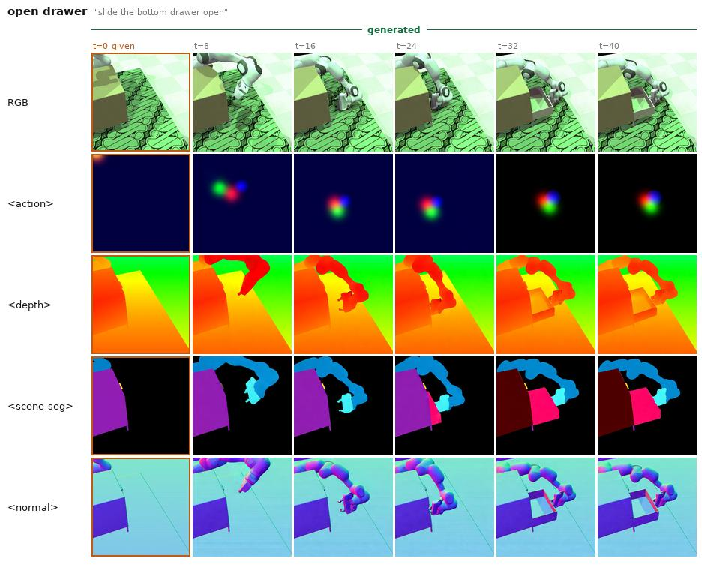
\includegraphics[width=\linewidth]{figures/scene_open_drawer.pdf}
\caption{\textbf{One checkpoint, four prompts.} All rows come from the same arm6 model, episode,
window and seed; only the prompt prefix differs (\ptag{video}\ptag{action},
\ptag{video}\ptag{depth}, \ptag{video}\ptag{scene-seg}, \ptag{video}\ptag{normal}). Columns are
frames of one $41$-frame, $6.0$\,s window, so each row is a filmstrip. Under \texttt{IIII}
conditioning only the first latent frame is given (orange, \texttt{t=0}); everything to its right
is generated. Instruction: \emph{``slide the bottom drawer open''}.}
\label{fig:qualitative}
\end{figure}
